\title{CS534 Implementation Assignment 1:\\Linear Regression, Perceptron}
\author{
        Amit Bawaskar, Michael Lam\\
        EECS, Oregon State University\\
        %\email{}
        %\and
}

\documentclass[12pt]{article}
\usepackage[english]{babel}
\usepackage{graphicx}
\usepackage{subfig}
\usepackage{amsmath}
\usepackage{hyperref}
\hypersetup{
    colorlinks,%
    citecolor=green,%
    filecolor=magenta,%
    linkcolor=red,%
    urlcolor=cyan
}

%\underset{x}{\operatorname{argmax}}
%\underset{x}{\operatorname{argmin}}
\DeclareMathOperator*{\argmin}{arg\,min}
\DeclareMathOperator*{\argmax}{arg\,max}

\begin{document}
\maketitle

\begin{abstract}
In this assignment, we implemented two versions of linear regression and perceptron, and compared their performance.
\end{abstract}

% -------------------------------------------------
\section{Introduction}
We implemented linear regression to solve the regression problem. Two versions were implemented and compared for performance: batch gradient descent and stochastic gradient descent. We also implemented two different versions of perceptron to solve the binary classification problem: batch perceptron and voted perceptron. Voted perceptron provides better behavior for the non-linearly separable case of training data.

\section{Linear Regression}
Linear regression learns a model that fits the training data in order to predict a target value for new data. This section compares the performance of our batch gradient descent and stochastic gradient descent algorithms for linear regression.

For both versions, our learning rate was set to the reciprocal of the number of training examples. Epsilon was set to \(.0001\). The termination criterion is if the L2 norm of the difference of the previous weight vector and the current weight vector is less than epsilon.

\subsection{Batch Gradient Descent}
For the batch gradient descent version, the following are results from training on the given training data set:

\begin{itemize}
	\item Learned weights: \([-0.3540, 0.5022, 2.2516, -0.5764]^T\)
	\item Sum of squared error on test data set: 0.775889
\end{itemize}

Figure \ref{fig:batchregerror} plots the sum of squared error vs. the number of training epochs. Notice a smooth curve. The batch gradient descent uses all training examples to calculate the gradient in one iteration. We will compare this with the stochastic gradient descent.

\begin{figure}[!t]
  \centering
  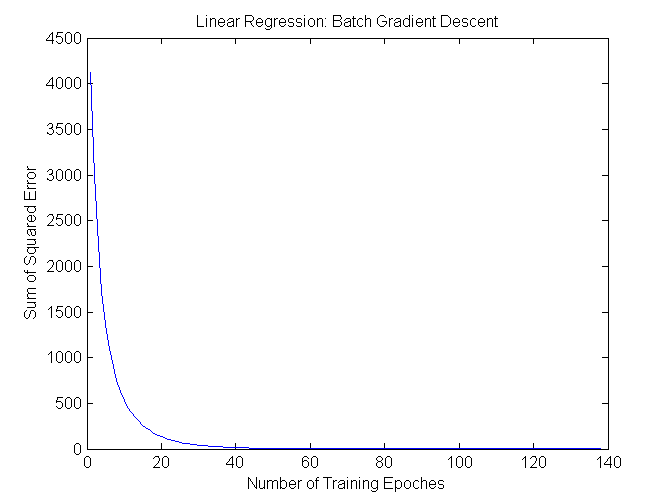
\includegraphics[scale=.70]{img/batch_regression_errors.png}
  \caption{Classification error of Linear Regression using Batch Gradient Descent}
  \label{fig:batchregerror}
\end{figure}

\subsection{Stochastic Gradient Descent}
For the stochastic gradient descent version, the following are results from training on the given training data set:

\begin{itemize}
	\item Learned weights: \([-0.3540, 0.5021, 2.2516, -0.5763]^T\)
	\item Sum of squared error on test data set: 0.775908
\end{itemize}

Observe that the weight vector obtained is very close in value to the weight obtained from batch gradient descent. The sum of squared error here is also slightly higher than the one for batch gradient descent.

Figure \ref{fig:stochregerror} plots the sum of squared error vs. the number of training epochs. Notice the curve is not smooth compared to the batch regression. In fact, it oscillates up and down. The stochastic version updates the gradient with each individual example. If the example is not good, then the error may increase at that time. However, the error decreases overall with time.

\begin{figure}[!t]
  \centering
  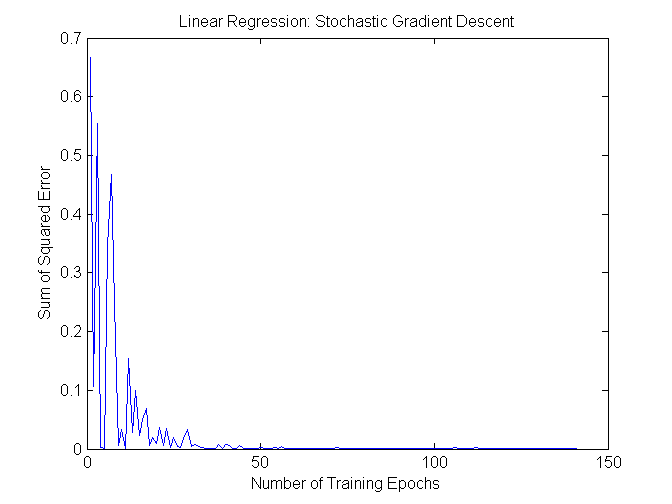
\includegraphics[scale=.70]{img/stochastic_regression_errors.png}
  \caption{Classification error of Linear Regression using Batch Gradient Descent}
  \label{fig:stochregerror}
\end{figure}

\section{Perceptron}

Perceptron is a linear classification model, which is used to create decision boundaries between various classes of the training data. Whenever new test data points are encountered, we can classify them according to the boundaries generated by the training data. This assignment focuses on binary classification. We have implemented two different types of Perceptron algorithms in this assignment, namely Batch Perceptron and Voted Perceptron.

\subsection{Batch Perceptron}

For the given dataset (twogaussian), the Batch Perceptron produced the following weights: \([99.0000, -41.5052, -34.4167]^T\)

Figure \ref{fig:batchpercepterror} plots the classification error vs. the number of training epochs. We notice a jagged descending function. It is jagged because perceptron updates the gradient with each misclassified example during the iteration. However, the number of classification examples eventually converges at zero and the algorithm terminates.

Figure \ref{fig:batchperceptscatter} plots the training data and the decision boundary learned from training. Since the data set is linearly-separable, batch perceptron terminates and provides a boundary that classifies all the data points correctly.

\begin{figure}[!t]
  \centering
  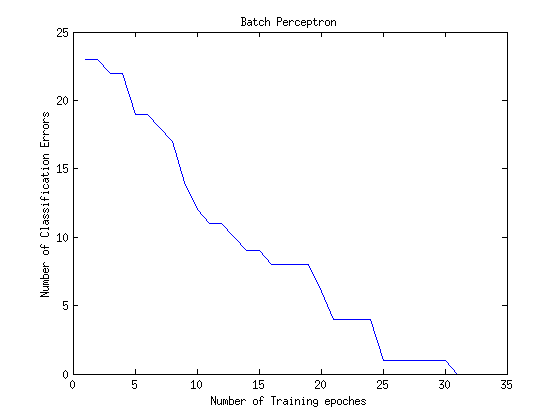
\includegraphics[scale=.70]{img/batch_errors.png}
  \caption{Classification error of Batch Perceptron}
  \label{fig:batchpercepterror}
\end{figure}

\begin{figure}[!t]
  \centering
  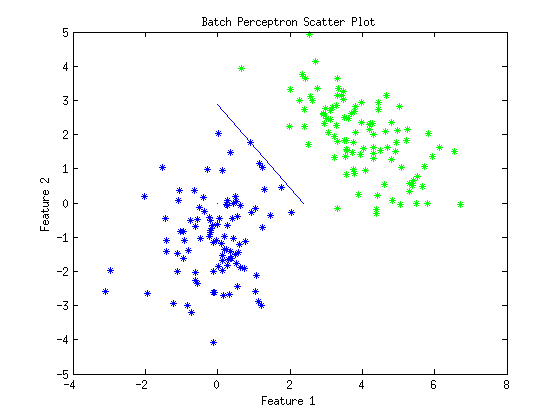
\includegraphics[scale=.70]{img/batch_scatterplot.png}
  \caption{Scatter Plot with decision boundary of Batch Perceptron}
  \label{fig:batchperceptscatter}
\end{figure}

\subsection{Voted Perceptron}

For the given dataset (iris-twoclass), the Voted Perceptron produced the following weights:

\begin{enumerate}
	\item Voted Perceptron without averaged weights:\\ \([126.0000, -15.2000, -43.7000]^T\)
	\item Voted Perceptron using averaged weights:\\ \([126.0000, -15.2000, -43.7000]^T\)
\end{enumerate}

Figure \ref{fig:votedpercepterror} plots the classification error vs. the number of training epochs. We notice an extremely jagged function. This is because we have a data set that is not linearly-separable, so regular perceptron would not converge. We terminate at 100 iterations.

The two learned weights of Voted Perceptron using averaged weights and without using averaged weights are equal, since the result of the stored weight method gets averaged out after every epoch. So the result of averaging all the weight vectors is equal to the result of storing all the weight vectors and calculating the class using that vector.

Figure \ref{fig:votedperceptscatter1} plots the training data and the decision boundary learned from training without using the averaged weight. Figure \ref{fig:votedperceptscatter2} plots the training data and the decision boundary learned from training when using the averaged weight.

\begin{figure}[!t]
  \centering
  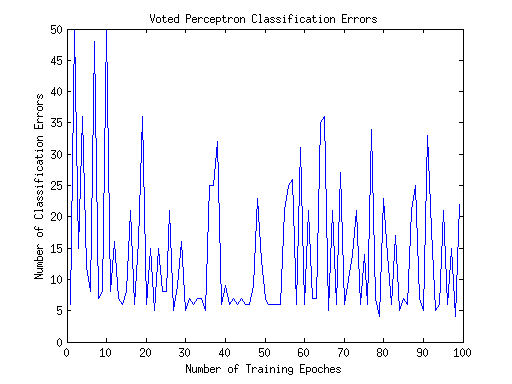
\includegraphics[scale=.70]{img/voted_errors.png}
  \caption{Classification error of Voted Perceptron}
  \label{fig:votedpercepterror}
\end{figure}

\begin{figure}[!t]
  \centering
  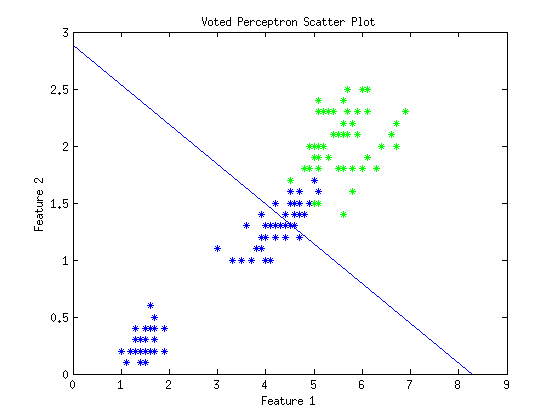
\includegraphics[scale=.70]{img/voted_scatterplot.png}
  \caption{Scatter Plot with decision boundary of Voted Perceptron}
  \label{fig:votedperceptscatter1}
\end{figure}

\begin{figure}[!t]
  \centering
  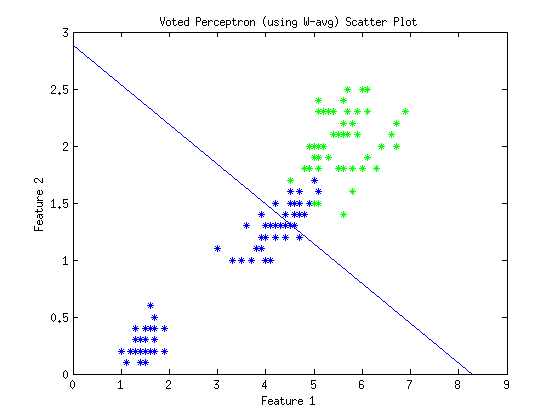
\includegraphics[scale=.70]{img/voted_avg_scatterplot.png}
  \caption{Scatter Plot with decision boundary of Voted Perceptron using  averaged weights}
  \label{fig:votedperceptscatter2}
\end{figure}

\end{document}
This is never printed
